\clearpage
\subsection{MSVC: x86 + \olly}
\myindex{\olly}

Il quadro qui è ancora più semplice:

\begin{figure}[H]
\centering
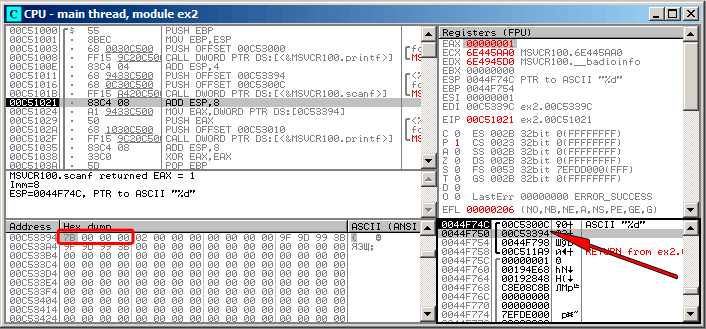
\includegraphics[scale=\FigScale]{patterns/04_scanf/2_global/ex2_olly_1.png}
\caption{\olly: after \scanf execution}
\label{fig:scanf_ex2_olly_1}
\end{figure}

La variabile è collocata nel data segment.
Dopo che l'istruzione \PUSH (che fa il push dell'indirizzo di $x$) viene eseguita, 
l'indirizzo appare nella finestra dello stack. Facciamo click destro su quella riga e selezioniamo \q{Follow in dump}.
La variabile apparirà nella finestra di memoria a sinistra.
Dopo aver inserito il valore 123 in console, 
\TT{0x7B} apparirà nella finestra della memoria (vedere regioni evidenziate nello screenshot).

Ma perchè il primo byte è \TT{7B}?
A rigor di logica, dovremmo trovare \TT{00 00 00 7B}.
La causa per cui troviamo invece \TT{7B} è detta \gls{endianness}, e x86 usa la convenzione \IT{little-endian}.
Ciò significa che il byte piu basso è scritto per primo, e quello più alto per ultimo.
Maggiori informazioni sono disponibili nella sezione: \myref{sec:endianness}.
Tornando all'esempio, il valore a 32-bit è caricato da questo indirizzo di memoria in \EAX e passato a \printf.

L'indirizzo in memoria di $x$ è \TT{0x00C53394}.

\clearpage
In \olly possiamo osservare la mappa di memoria di un processo  (process memory map, Alt-M)
e notare che questo indirizzo è dentro il segmento PE \TT{.data} del nostro programma:

\begin{figure}[H]
\centering
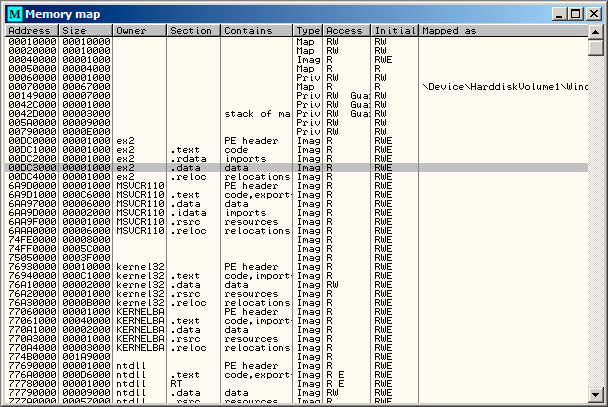
\includegraphics[scale=\FigScale]{patterns/04_scanf/2_global/ex2_olly_2.png}
\caption{\olly: process memory map}
\label{fig:scanf_ex2_olly_2}
\end{figure}

